\documentclass{article} % For LaTeX2e
\usepackage{nips12submit_e,times}
\nipsfinalcopy % Uncomment for camera-ready version
\usepackage{graphicx}
\usepackage{amsmath}
\usepackage{amssymb}
\usepackage{amsthm}
\usepackage{hyperref}
\usepackage{natbib}
\usepackage{caption}
\usepackage{subcaption}


\newcommand{\B}[1]{{\bf #1}}
\newcommand{\Sc}[1]{{\mathcal{#1}}}
\newcommand{\R}[1]{{\rm #1}}
\newcommand{\mB}[1]{{\mathbb{#1}}}
%%%%%%%%%%%%%%%%%%%%%%%%%
% Commands copied from hart.sty
\newcommand{\bB}{\bf{B}}\newcommand{\bN}{\bf{N}}
% \newcommand{\B{1}}{\mathbb {1}}
%%%%%%%%%%%%%%%%%%%%%%%%%


% Macros added by Burke
\newcommand{\set}[2]{\left\{#1\,\left\vert\, #2\right.\right\}}
\newcommand{\one}{\bf{1}}
\newcommand{\half}{\frac{1}{2}}
\newcommand{\map}[3]{#1\,:\,#2\rightarrow #3}
\newcommand{\cS}{\mathcal{S}}
\newcommand{\cL}{\mathcal{L}}




\newtheorem{lemma}{Lemma}[section]
%\newtheorem{remark}{Remark}[section]
\newtheorem{remark}[lemma]{Remark}
\newtheorem{theorem}[lemma]{Theorem}
\newtheorem{corollary}[lemma]{Corollary}
\newtheorem{conjecture}[lemma]{Conjecture}
\newtheorem{proposition}[lemma]{Proposition}
\newtheorem{definition}[lemma]{Definition}
\newtheorem{algorithm}[lemma]{A}

\title{Sparse Coding for Dictionary Learning in Context of Image De-noising}


\author{
Dhaivat Deepak Shah\\
\texttt{ds3267@columbia.edu} \\
\And
Gaurav Ahuja\\
\texttt{ga2371@columbia.edu} \\
\And
Sarah Panda\\
\texttt{sp3206@columbia.edu} \\
}

% The \author macro works with any number of authors. There are two commands
% used to separate the names and addresses of multiple authors: \And and \AND.
%
% Using \And between authors leaves it to \LaTeX{} to determine where to break
% the lines. Using \AND forces a linebreak at that point. So, if \LaTeX{}
% puts 3 of 4 authors names on the first line, and the last on the second
% line, try using \AND instead of \And before the third author name.

\newcommand{\fix}{\marginpar{FIX}}
\newcommand{\new}{\marginpar{NEW}}

%\nipsfinalcopy % Uncomment for camera-ready version

\begin{document}


\maketitle


\begin{abstract}
Sparse Coding is the modeling of data vectors as linear combination of basis elements or atoms which form the Dictionary. In this paper we study the behaviour of various sparse coding algorithms when used in K-SVD for Dictionary learning. Dictionary learning technique has been used to denoise an image by learning a dictionary from the noisy image. We learn dictionaries of various sizes for images with varying levels of noise and compare the performance of various sparse coding algorithms in-terms of time per iteration and the SNR of the denoised image resulting from the dictionary learnt using these algorithms.
\end{abstract}

\vspace{-.2cm}
\section{Introduction}
\vspace{-.2cm}
Image restoration is a widely studied problem in image processing and the common approaches to solve the problem include filtering, minimizing variations in an image etc. The problem we address in this paper is to remove noise from a given image using Dictionary Learning approach, assuming the noise to be Gaussian and additive. The approach bases itself on representing an image as a sparse representation over a good dictionary. So our problem of restoring images boils down to learning a good dictionary and finding a good representation of any given patch of an image using the dictionary. Designing dictionaries to better the above model can be done by either selecting one from a pre-specified set of linear transforms, or by adapting the dictionary to a set of training signals. Past research has shown that dictionaries adapted to training signals lead to a lot better signal restoration than the pre-specified dictionaries. Hence, we strive to learn a dictionary from the input signals for the purpose of restoration. We have used the K-SVD algorithm as our basis for dictionary learning and explore different sparse coding methods that can be used for the same. The next section gives a Literature review of the different components of Dictionary Learning. The third section talks about our experimental setting and further sections discuss the results, our analysis and conclusion. 

\section{Intro to Dictionary learning}
Dictionary Learning is a focus area in the Signal Processing domain. A dictionary is used for the sparse representation or approximation of signals. A dictionary $D$, is an $NxK$ matrix that contains $K$ prototype signals called atoms. A signal $y_0$ can be represented by a linear combination of a small number of these atoms. For any signal $y_0$ and dictionary $D$ there must exist a sparse vector $x \in R^K$ such that:
\begin{align}
y_0 = D*x
\end{align}   
There will be cases where we cannot exactly represent the signal with a linear combinations of atoms from a finite dictionary. In such a case we find an approximation of the signal, $y$ such that:
\begin{align}
y = D*x \\
\|y - y_0\| < \epsilon
\end{align} 
Dictionary Learning is a problem of finding a dictionary such that the approximation of many vectors in the training set are as good as possible. 

For a finite number of training vectors, $L$ each of length $N$ the aim of Dictionary Learning is to find both a Dictionary $D$, of size $NxK$ and the $L$ corresponding coefficients vectors of length $K$.

In this paper we will apply the problem of Dictionary Learning on noisy image. The image is broken into $8x8$ pixel patches and this $N = 64$ pixel vector is approximated by the linear combination of atoms of the Learned Dictionary.


\subsection{Problem Statement}
Classical dictionary learning techniques consider a finite training set of signals $Y = [y_1, y_2, \ldots, y_L]$ int $R^{NxL}$ and optimize the empirical cost function:
\begin{align}
f(D) &= \frac{1}{L}\sum_{i=1}^{L}l(y_i, D)
\end{align} 
where $D \in R^{NxK}$ is the dictionary and $l$ is the loss function such that $l(y,D)$ is small if $D$ is a good at representing the signal $x$. 

$l(y,D)$ can be define as the optimal value of the $l_1$ or $l_0$ sparse coding problem. See section on Sparse coding for more details, TODO: rephrase this. We consider the $l_1$ norm for illustration in this section.
\begin{align}
l(y, D) = \min_{x \in R^K} \frac{1}{2}\|y - Dx\| + \lambda \|x\|_1
\end{align}
$\lambda$ is the regularization parameter. The problem of minimizing the empirical cost function $f(D)$ is not convex with respect to $D$. It can be rewritten as a joint optimization problem with respect to dictionary $D$ and the coefficients $x = [x_1, x_2, \ldots, x_L]$, which is not jointly convex, but convex with respect to each of the two variables $D$ and $x$ when the other one is fixed.
\begin{align}
\min_{D\in R^{NxK}, x\in R^{KxL}} \frac{1}{L}\sum_{i=1}^{L} \left( \frac{1}{2}\|y_i - Dx_i\|^2_2 + \lambda \|x\|_1 \right)
\end{align} 
A natural approach to solving this problem is to alternate between the two variables, minimizing one over the other while keeping the other fixed. 
 

\section{K-SVD for dictionary learning}

The goal of K-SVD is to adapt a dictionary to the training signals such that it ensures the best sparse representation for each of the signals, under constraints of reconstruction error and sparsity. It is a two-step iterative process, which begins with a dictionary initialization.  The dictionary could be initialized with any pre-calculated well known dictionary, like DCT, or created from the noisy image by randomly selecting atoms from the patches of the given image. 
The first step of the process determines the sparse code for the given training signals with fixed dictionary. The second step assumed fixed sparse code and updates the dictionary to better fit the data. The second step further updates the sparse representation of the training signals to accelerate convergence. \\ \\
K-SVD tries to optimize the following overall MSE under sparsity constraints in each iteration:\\
\begin{center}
$\min\limits_{d,x}{\|Y-DX\|_F}^2$ subj. to, $\forall i, \|x_i\|_0<=L$
\end{center}
The algorithm is outlined below:\\

\begin{enumerate}
\item $\textbf{Initialization:}$  Set dictionary matrix $D  \in R^{nXK}$ with $l_2$ normalized columns
\item $\textbf{while}$ not converged($j$ = 1,2,\ldots) \textbf{do}
\item \hspace*{.4cm} $\textbf{Sparse Coding:}$ 
\item \hspace*{.8cm}Compute $x_i$ for every training signal $y_i$, by solving for\\
\hspace*{.8cm}$\min_{x_i}{{\|y_i-Dx_i\|}_F}^2$ subject to $\|x_k\|_0\leq L$
\item \hspace*{.4cm} $\textbf{Dictionary Update:}$ 
\item \hspace*{.8cm} Update each atom k in {1,2,..K} in $D_{j-1}$ as below:
\begin{enumerate}
\item \hspace*{.8cm} Let $w_k$ be the set of input signals that use this atom D(k).
\item \hspace*{.8cm} Find the overall error in representation, in matrix $E_k$,\\
\hspace*{.8cm} $E_k = Y - \sum(j \neq k){d_j{x_j}^2}$
\item \hspace*{.8cm} Restrict $E_k$ by choosing columns corresponding to $w_k$ as $E_k^R$
\item \hspace*{.8cm} Apply SVD decomposition on the restricted error matrix :\\
\hspace*{.8cm}$E_k^R = U\delta V^T$\\
\hspace*{.8cm}Set $d_k = U[:1]$\\
\hspace*{.8cm}and $x_r^k = V[:1]*\delta(1,1)$
\end{enumerate}
\item \hspace*{.8cm}j= j+1
\item \textbf{end while}
\item \textbf{Output: } $X^{*} \leftarrow X_j, D^{*} \leftarrow D_j$
\end{enumerate}


In this paper, we focus on the first step of K-SVD and that is the sparse coding step. The following sections discuss the problem of sparse coding in detail along with the algorithms we have used.
\section{Sparse Coding}
As mentioned before, any signal y can be represented as a linear combination of atoms in a dictionary D. Sparse coding problem aims at finding the sparsest such representation. On a high level, those atoms summarize the most important features in the input.\\
\begin{center}
$\min\|x\|_0$  subj. to $y=Dx$
\end{center}
The above equation tries to find the sparsest coefficient vector that exactly reconstructs the input signal. However, this form of exact determination is NP-hard. So, to make it easier to solve, the problem needs to be relaxed by allowing for a small amount of reconstruction error, $\epsilon$. The problem can be thus formulated as,\\
\begin{center}
$\min\|x\|_0$  subj. to $\|y-Dx\| \leq \epsilon$
\end{center}
Still the problem is computationally expensive and following are two of the well known approaches to approximate the solution to the above.



\subsection{Greedy (Matching pursuit)}
Greedy methodology, solves the problem in (2) by sequentially selecting the atom that best explains the data. The coefficient vector(sparse code) is then updated to include the selected atom and its contribution to the signal is deducted from the residual. Upon convergence, the coefficient vector assumes a sparse code for the input signal over the given dictionary. We cover two important Greedy algorithms, Matching Pursuit and Orthogonal Matching pursuit in the section below and also, study their performance in K-SVD de-noising.

\subsection{Relaxation (Basis pursuit)}

In the relaxation methodology, the $l_0$ norm in (2) is replaced with the $l_1$ norm, resulting in the following equivalent objective,

\[\min{\|y-Dx\|}^2 +\lambda \|x\|_1\]

L1 regularization penalizes the non-sparse terms based on their actual values, which may seem unfair, but past research has shown that it leads to a very good approximation and often leads to the sparsest representation.  The resulting optimization problem is convex and unconstrained, and hence can be solved using several methods like gradient descent.



\section{Summary of sparse coding techniques used:}

\subsection{MP}
  Matching pursuit, proposed by Mallat and Zhang et al \citep{mallat1993matching} is a well known greedy algorithm for learning sparse code of a signal over a given dictionary. The basic idea of the algorithm is outlined below.\\ 
At every step of refining the sparse code, the algorithm picks an atom of the dictionary that best represents a portion of the input signal. \\

The following pseudo-code briefly describes the algorithm:\\


\begin{enumerate}
\item \textbf{Input:} Training signal – y, Dictionary - D
\item \textbf{Initialization:} $R_1=y$, $x=0, n=1$
\item $\textbf{while}$ $R_n >$ Threshold \textbf{do}
\item \hspace*{.4cm} Find $d_i \in $ D with max correlation with residual i.e. $<R_n,d_i>$
\item \hspace*{.4cm} $x_i=x_i+<R,d_i>$
\item \hspace*{.4cm} $R_{n+1}=R_n-x_id_i$
\item \hspace*{.4cm} $n=n+1$
\item \textbf{end while}
\item \textbf{Output: }Sparse code of y over D, $x^* \leftarrow x_n$
\end{enumerate}

           The algorithm evaluates the best matching atom at every step by evaluating the inner product between the Residual, $R_n$ and the individual atoms from the dictionary. The coefficient vector x is updated with the atom that has maximum inner product and its contribution to the signal is deducted from the signal. The process repeats until the residual falls below a threshold. The sparse coefficients thus learned is believed to be the sparsest approximation of the decomposition of the signal over the dictionary.

\subsection{OMP}
A variation of the Matching Pursuit is the Orthogonal Matching Pursuit \citep{pati1993orthogonal}, also a greedy method that iteratively selects the atom having highest correlation with the residual. The difference is that after adding the best matched atom to the coefficient vector, the residual is updated with the orthogonal projection of the input signal y onto the subspace of previously selected atoms. This set of selected atoms is called the active set and since the resulting residual is orthogonal to each of the atoms in the set, none of those atoms are selected in the future iterations. \\

The OMP algorithm is as below:

\begin{enumerate}
\item \textbf{Input:} Training signal – y, Dictionary - D
\item \textbf{Initialization:} $R_0=y$, $X(c_0)=0, n=0$
\item $\textbf{while}$ not converged \textbf{do}
\item \hspace*{.4cm} Solve for $X_{t_i}$ by minimizing,\\
\hspace*{.4cm} $\max_t{{X_t}^TR_{n-1}}$\\
\hspace*{.4cm} Add $X_{t_i}$ to the set of selected atoms; $c_n = c_{n-1}\cup {t_i}$
\item \hspace*{.4cm} Let $P_n = X(c_n){(X(c_n)^TX(c_n))}^{-1}{X(c_n)}^T$ denote the projection onto the linear space spanned by the elements of $X(c_n)$. 
\item \hspace*{.4cm} Update $R_n = (I - P_n)y$.
\item \hspace*{.4cm} $n=n+1$
\item \textbf{end while}
\item \textbf{Output: }Sparse code of y over D, $x^* \leftarrow x_n$
\end{enumerate}


\vspace{.2cm}
\subsection{FISTA}
\vspace{.2cm}
The objective function that we have as defined above is:
\begin{center}
$F(x) = \frac{1}{2}\|y - Dx\|^2 + \lambda\|x\|_1$
\end{center}

Here the first term, $f(x)$ is a smooth, convex function with Lipschitz continuous gradient $D^T(Dx - y)$ and $L_f = \|D^TD\|$.

FISTA, proposed by Beck \citep{beck2009fast} has a faster convergence rate as compared to ISTA. The main difference between the two is that the iterative shrinkage operator is not applied to the previous point alone but to another point which uses a specific linear combination of the previous two points. The algorithm in this case becomes:

\begin{enumerate}
\item \textbf{Input: }$L_f$
\item \textbf{Step 0. }$j_1 = x_0$ $\epsilon$ $\mathbb{R}^n, t_1 = 1$
\item \textbf{Step $k$.}($k \geq 1$)
\item \hspace{.4cm} $x_k = soft(j_k - \frac{1}{L_f}\nabla f(j_k), \frac{\lambda}{L_f})$
\item \hspace{.4cm} $t_{k+1} = \frac{1+\sqrt{1+4t_k^2}}{2}$
\item \hspace{.4cm} $y_{k+1} = x_k + \frac{t_k-1}{t_k+1}(x_k - x_{k-1})$
\end{enumerate}


  
\vspace{-.2cm}
\subsection{ALM}
\vspace{-.2cm}

The Augmented Lagrangian Method was proposed individually by Powell \citep{powell1964efficient} and Hestenes \citep{hestenes1969multiplier} and is explained in depth by Nocedal, Wright \citep{wright1999numerical}. It is an extension to the quadratic penalty function method proposed by Courant \citep{courant1943variational}. In the penalty function method, we add a quadratic penalty term for each of the constraints in a constrained optimisation problem. That is for:
\begin{center}
$\min\limits_x f(x)$ subj. to $c(x) = 0$
\end{center}
the formulation becomes,
\begin{center}
$\min\limits_x f(x) + \frac{\mu}{2}\|c(x)\|^2$
\end{center}
where $\mu$ is the penalty parameter and is always positive. We can now progressively increase $\mu$ towards $\infty$ and try to find a minimizer for the objective function.
Thus we can convert the constrained minimisation problem into an unconstrained one. However, an ill-conditioning for the Hessian in the formulation can lead to significantly poor results for the iterative methods. To reduce this possibility, we include a Lagrange multiplier to get the Augmented Lagrangian as:
\begin{center}
$\min\limits_x f(x) + \frac{\mu}{2}\|c(x)\|^2 + \lambda c(x)$
\end{center}

We look at both the primal and the dual formulations of this approach.

\vspace{-.2cm}
\subsubsection{Primal ALM}
\vspace{-.2cm}
In our case, the problem boils down to:
\begin{center}
$L_{\mu}(x,e,\lambda) = \|x\|_1 + \|e\|_1 + \frac{\mu}{2}\|y - Dx - e\|^2 + \lambda (y - Dx - e)$
\end{center}

For the primal problem, Bertsekas \citep{bertsekasnonlinear} showed that there exists a $\lambda^{*}$ and $\mu^{*}$ such that
\begin{center}
\begin{align*}
e_{k+1} &= arg \min_e L_{\mu}(x_k,e,\lambda_k)\\
x_{k+1} &= arg \min_x L_{\mu}(x,e_{k+1},\lambda_k)\\
\lambda_{k+1} &= \lambda_k + \mu(y - Dx_{k+1} - e_{k+1})
\end{align*}
\end{center}

Of the above equations, the one for $e$ has a closed form solution. As for the update of $x$, it is a standard $L_1$ minimisation problem which we solve using the FISTA method explained above.

So the overall algorithm can be summarized as in \citep{yang2010fast}:

\begin{enumerate}
\item $\textbf{Input:}y$ $\epsilon$ $\mathbb{R}^m,$ $D$ $\epsilon$ $\mathbb{R}^{mxn},$ $x_1 = 0,$ $e_1 = y,$ $\lambda_1 = 0$
\item $\textbf{while}$ not converged($k$ = 1,2,\ldots) \textbf{do}
\item \hspace*{.4cm} $e_{k+1} \leftarrow shrink(y - Dx_k + \frac{1}{\mu}\lambda_k, \frac{1}{\mu})$
\item \hspace*{.4cm} $t_1 \leftarrow 1, z_1 \leftarrow x_k, w_1 \leftarrow x_k$
\item \hspace*{.4cm} $\textbf{while}$ not converged ($l$ = 1,2,\ldots) \textbf{do}
\item \hspace*{.8cm} $w_{l+1} \leftarrow shrink(z_l + \frac{1}{l}D^T(y - Dz_1 - e_{k+1} + \frac{1}{\mu}\lambda_k),\frac{1}{\mu L})$
\item \hspace*{.8cm} $t_{l+1} \leftarrow \frac{1}{2}(1 + \sqrt{1+4t_l^2})$
\item \hspace*{.8cm} $z_{l+1} \leftarrow w_{l+1} + \frac{t_l - 1}{t_l + 1}(w_{l+1} - w_l)$
\item \hspace*{.4cm} \textbf{end while}
\item \hspace*{.4cm} $x_{k+1} \leftarrow w_l, \lambda_{k+1} \leftarrow \lambda_k + \mu(y - Dx_{k+1} - e_{k+1})$
\item \textbf{end while}
\item \textbf{Output: } $x^{*} \leftarrow x_k, e^{*} \leftarrow e_k$
\end{enumerate}

While in the general case of Augmented Lagrangian methods, the value of $\mu$ is incremented after every iteration, we are holding it fixed to the initialisation value.

\vspace{-.2cm}
\subsubsection{Dual ALM}
\vspace{-.2cm}
The dual Augmented Lagrangian method for efficient sparse reconstruction was proposed by Tomioka  \citep{tomioka2009dual}. It tries to solve the dual of the problem we have been tackling so far as:

\begin{center}
$\max\limits_j y^Tj$ subj. to $D^Tj$ $\epsilon$ $\mathbb{B}_1^\infty$
\end{center}
where $\mathbb{B}_1^\infty = \{x$ $\epsilon$ $\mathbb{R}^n : \|x\|_\infty \leq 1\}$

The associated Lagrangian function becomes:
\begin{center}
$\min\limits_{j,z} -y^Tj - \lambda^T(z-D^Tj) + \frac{\mu}{2}\|z-D^Tj\|^2$ subj. to $z$ $\epsilon$ $\mathbb{B}_1^\infty$
\end{center} 

Here, again there is a simultaneous minimization w.r.t. j,$\lambda$ and z. So we adopt an alternation strategy to get the following algorithm as in \citep{yang2010fast}:

\begin{enumerate}
\item \textbf{Input:} $y$ $\epsilon$ $\mathbb{R^m}, B = [A,I]$ $\epsilon$ $\mathbb{R}^{mx(n+m)}, w_1 = 0, j_1 = 0$
\item \textbf{while} not converged ($k$ = 1,2,\ldots) \textbf{do}
\item \hspace{.4cm} $z_{k+1} = \mathbb{P}_{\mathbb{B}_1^\infty}(B^Tj_k + \frac{w_k}{\mu})$
\item \hspace{.4cm} $j_{k+1} = (BB^T)^{-1}(Dz_{k+1} - (Bw_k - y)/\mu)$
\item \hspace{.4cm} $w_{k+1} = w_k - \mu(z_{k+1} - D^Tj_{k+1})$
\item \textbf{end while}
\item \textbf{Output: }$\lambda^{*} \leftarrow w_k[1:n], e^{*} \leftarrow w_k[n+1:n+m], j^{*} \leftarrow j_k$
\end{enumerate}

\subsection{Feature Sign}
Feature sign aims to solve the following L-1 regularized sparse coding problem
\begin{align}
\min_x f(x) = \|y - Dx\|^2 + \lambda\|x\|_1
\end{align}
The intuition behind this algorithm is that if we know the signs(positive, negative or zero) of $x_i$ at the optimal value we can replace $\|x_i\|$ by either $x_i$ if $x_i > 0$, $-x_i$ if $x_i < 0$ or 0 if $x_i = 0$. Considering only non zero coefficients this problem reduces to a standard quadratic optimization problem. This problem can them be solved analytically and efficiently. Feature sign algorithm tries to search for the signs of the coefficients. Given any such search results, it efficiently solves the resulting unconstrained quadratic problem. Further the algorithm systematically refines the guess if it turns out to be initially incorrect.

\begin{enumerate}
\item \textbf{Initialize} $x := 0$, $\theta : 0$ and active set $:= \{\}$, $\theta_i \in \{-1,0,1\}$ denotes sign($x_i$)
\item From zero coefficients of $x$, select $i = $ arg$\max_i |\frac{\partial\|y - Dx\|^2}{\partial x_i}|$\\
Activate $x_i$ (add $i$ to active set) only if it locally improves the objective
\begin{enumerate}
\item If $|\frac{\partial\|y - Dx\|^2}{\partial x_i}| > \lambda$; set $\theta_i := -1$, active set $:= \{i\} \cup$active set
\item If $|\frac{\partial\|y - Dx\|^2}{\partial x_i}| < -\lambda$; set $\theta_i := 1$, active set $:= \{i\} \cup$active set
\end{enumerate}
\item \textbf{Feature-Sign step:}\\
Let $\hat{D}$ be a submatrix of $D$ that contains only the columns corresponding to the active set.\\
Let $\hat{x}$ and $\hat{\theta}$ be sub vectors of $x$ and $\theta$ corresponding to the active set.\\
Compute the analytical solution to the resulting quadratic problem\\
$\hat{x}_{new} := (\hat{D}^T\hat{D})^{-1}(\hat{D}^Ty - \lambda \hat{\theta}/2)$\\
Perform a discrete line search on the closed line segment from $\hat{x}$ to $\hat{x}_{new}$:\\
- Check the objective value at $\hat{x}_{new}$ and all points where any coefficient changes sign.\\
- Update $\hat{x}$ (and all corresponding entries in $x$) to the point with the lowest objective value\\
Remove zero coefficients of $\hat{x}$ from the active set and update $\theta := $sign($x$)
\item \textbf{Check the optimality conditions}:
\begin{enumerate}
\item Optimality condition for nonzero coefficients: $|\frac{\partial\|y - Dx\|^2}{\partial x_i}| + \lambda$sign($x_i$) $=  0$ $\forall x_i \neq 0$\\
If this condition is not satisfied, go to Step 3(without any new activation); else check condition (b).
\item  Optimality condition for zero coefficients: : $|\frac{\partial\|y - Dx\|^2}{\partial x_i}| + \lambda$sign($x_i$) $\leq 0$ $\forall x_i = 0$\\
If this condition is not satisfied go to Step 3; otherwise return $x$ as the solution.
\end{enumerate} 
\end{enumerate}



\subsection{TNIPM}
In \cite{l1lskim2007efficient}, the authors formulate a Truncated Newton Interior Point method. The algorithm solves the L-1 regularised problem:
\begin{align}
\min_x f(x) = \|y - Dx\|^2 + \lambda\|x\|_1
\end{align}
This problem can be transformed to a convex quadratic program with linear inequality constraints,
\begin{align}
\min \|y - Dx\|^2 + \sum_{i= 1}^{K}\lambda u_i	\\
\text{subject to:} -u_i \leq x_i \leq u_i, \forall i \in \{i,K\}
\end{align}
The aim of this algorithm is to solve this quadratic program using the Newton's method. Since solving the Newton system exactly is computationally expensive for large L-1 problems, TNIPM uses an iterative method, Preconditioned Conjugate Gradient (PCG) to approximately solve the Newton system and develops an interior point method to solve the L-1 problem. 

\vspace{.2cm}
\section{Experimental Setup}
\vspace{.2cm}
We have used the K-SVD approach suggested in the previous sections for Dictionary Learning, and have used above mentioned 7 solvers for benchmarking.
The dictionary has been initialised with a DCT dictionary in each of the cases.

8 iterations of K-SVD were performed.
For each of the solvers, the following parameters have been varied:
\begin{enumerate}
\item Starting Image Noise Levels: 10, 20, 50 dB
\item Dictionary Size: 64, 128, 256
\end{enumerate}

And the comparison is based on:
\begin{enumerate}
\item Execution Time
\item SNR of the de-noised image
\end{enumerate}

All other supplied parameters were fixed across approaches, although tuning them specifically to a particular method might have resulted in better results, in order to maintain consistency across the experiment.

K-SVD toolbox \citep{rubinstein2008efficient} and L1 Solvers \citep{yang2010fast}, \citep{lee2007efficient} were used for computation, and all the processes were run using matlab in nodesktop mode.

Pertinent values, images and dictionaries at each of the intermediate steps were recorded and are hosted at \href{https://github.com/dkdfirefly/aml}{AML Project Results} under the respective results folders.

\vspace{.2cm}
\section{Findings}
\vspace{.2cm}
The following figures show our results

\begin{figure*}[h]
        \centering
        \begin{subfigure}[b]{0.5\textwidth}
                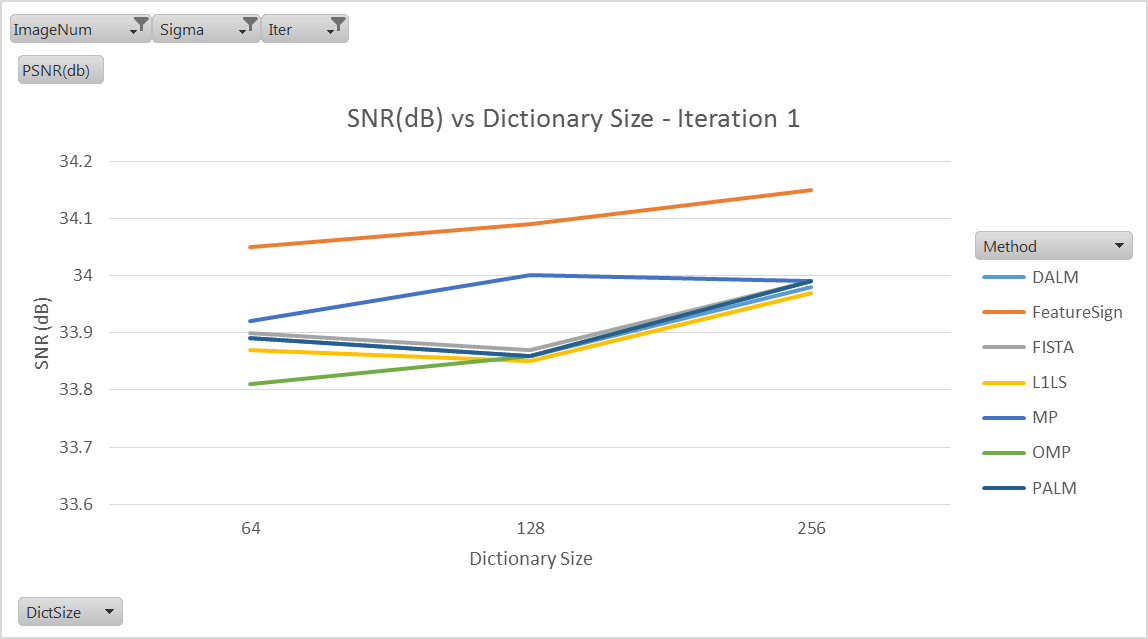
\includegraphics[width=\textwidth]{images/graph1}
                \caption{Iteration 1}
                \label{fig:dictSizeVar1}
        \end{subfigure}%
        ~ %add desired spacing between images, e. g. ~, \quad, \qquad etc.
          %(or a blank line to force the subfigure onto a new line)
        \begin{subfigure}[b]{0.5\textwidth}
                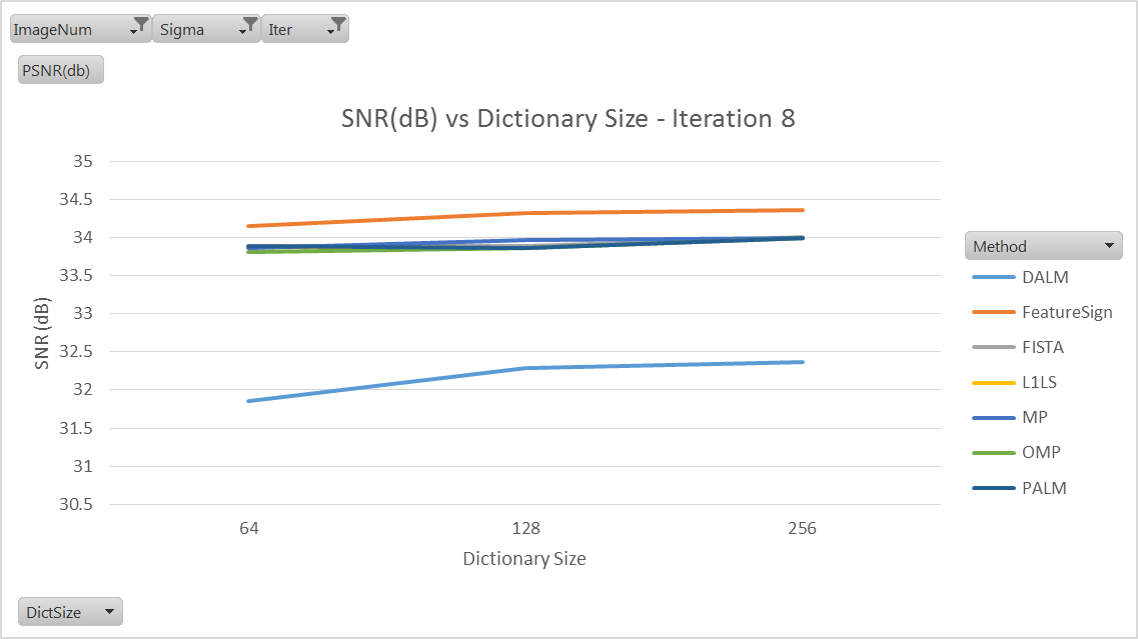
\includegraphics[width=\textwidth]{images/graph2}
                \caption{Iteration 8}
                \label{fig:dictSizeVar8}
        \end{subfigure}
        \caption{Variation with Dictionary Size}\label{fig:dictSizeVar}
\end{figure*}

\begin{figure*}[h]
        \centering
        \begin{subfigure}[b]{0.5\textwidth}
                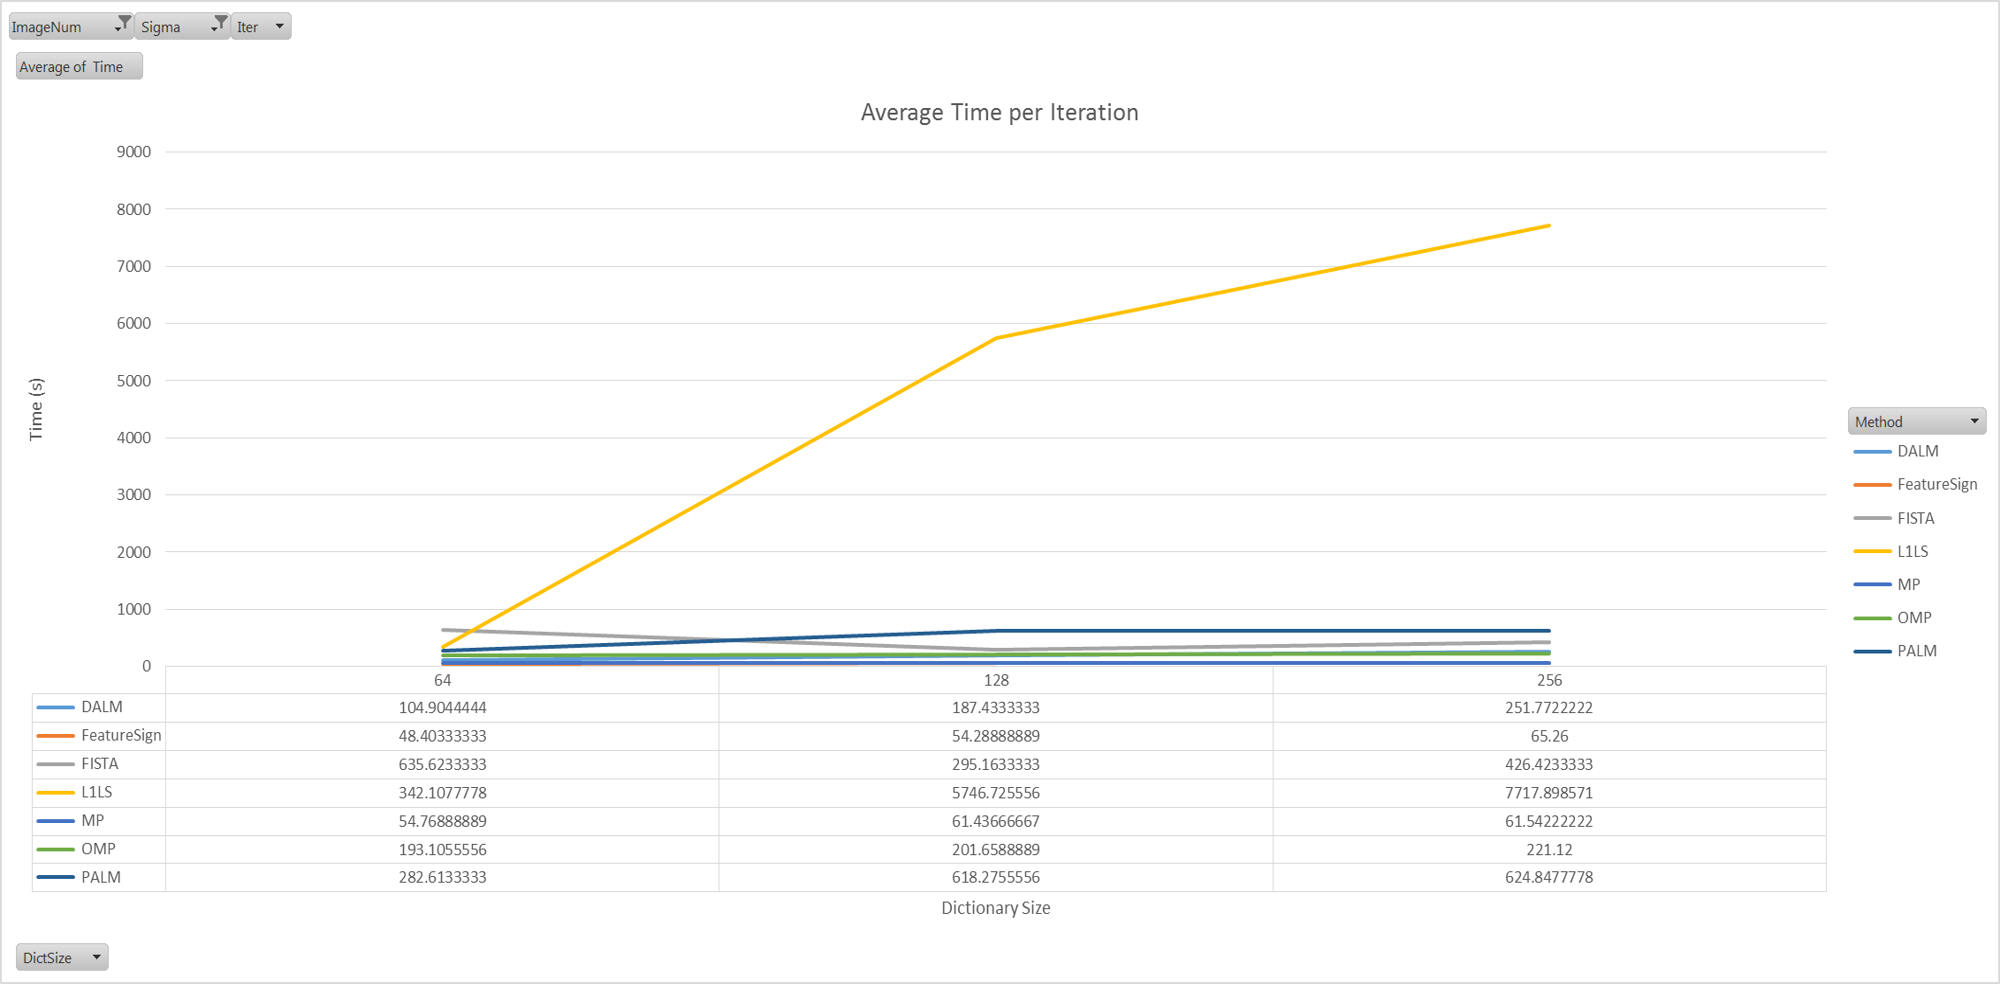
\includegraphics[width=\textwidth]{images/graph3}
                \caption{Average Time per iteration}
                \label{fig:avgTime}
        \end{subfigure}%
        ~ %add desired spacing between images, e. g. ~, \quad, \qquad etc.
          %(or a blank line to force the subfigure onto a new line)
        \begin{subfigure}[b]{0.5\textwidth}
                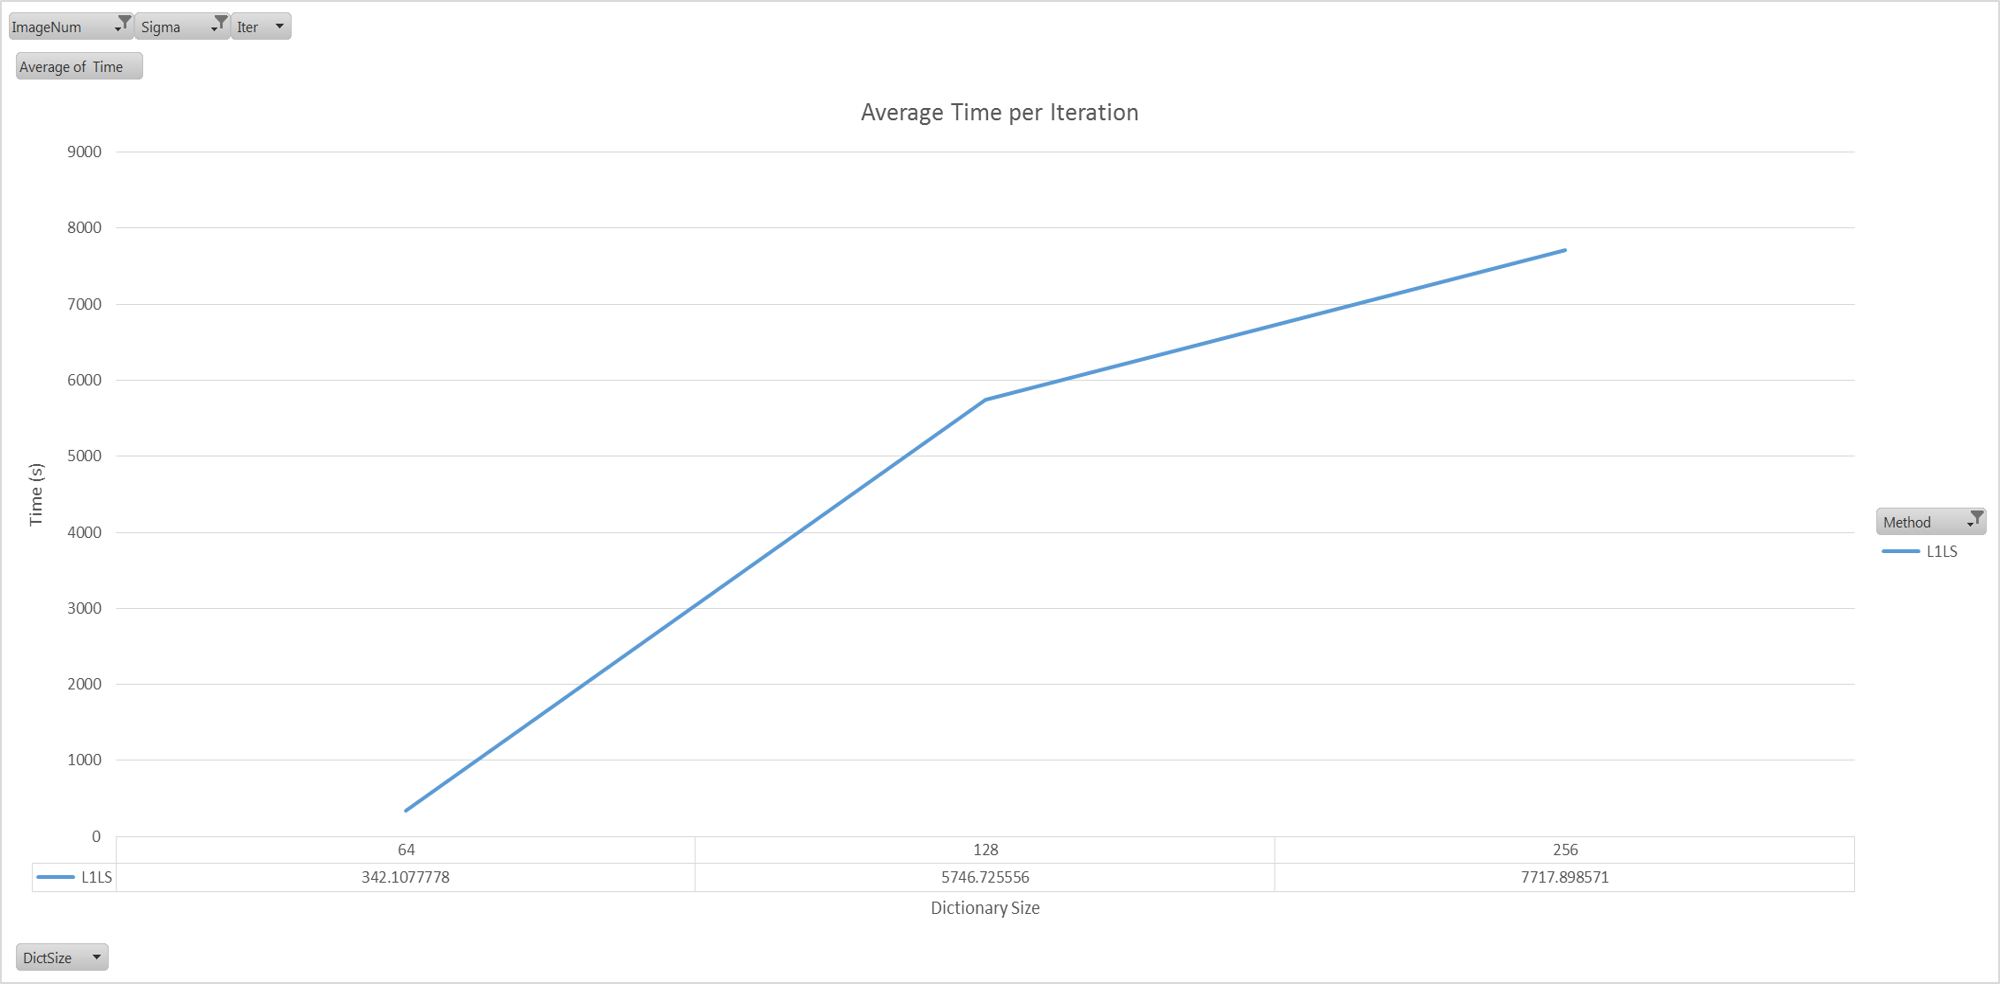
\includegraphics[width=\textwidth]{images/graph4}
                \caption{Average Time per iteration for L1LS}
                \label{fig:avgTimeL1LS}
        \end{subfigure}
        \caption{Avg Execution Time}\label{fig:avgExecTime}
\end{figure*}

\begin{figure*}
	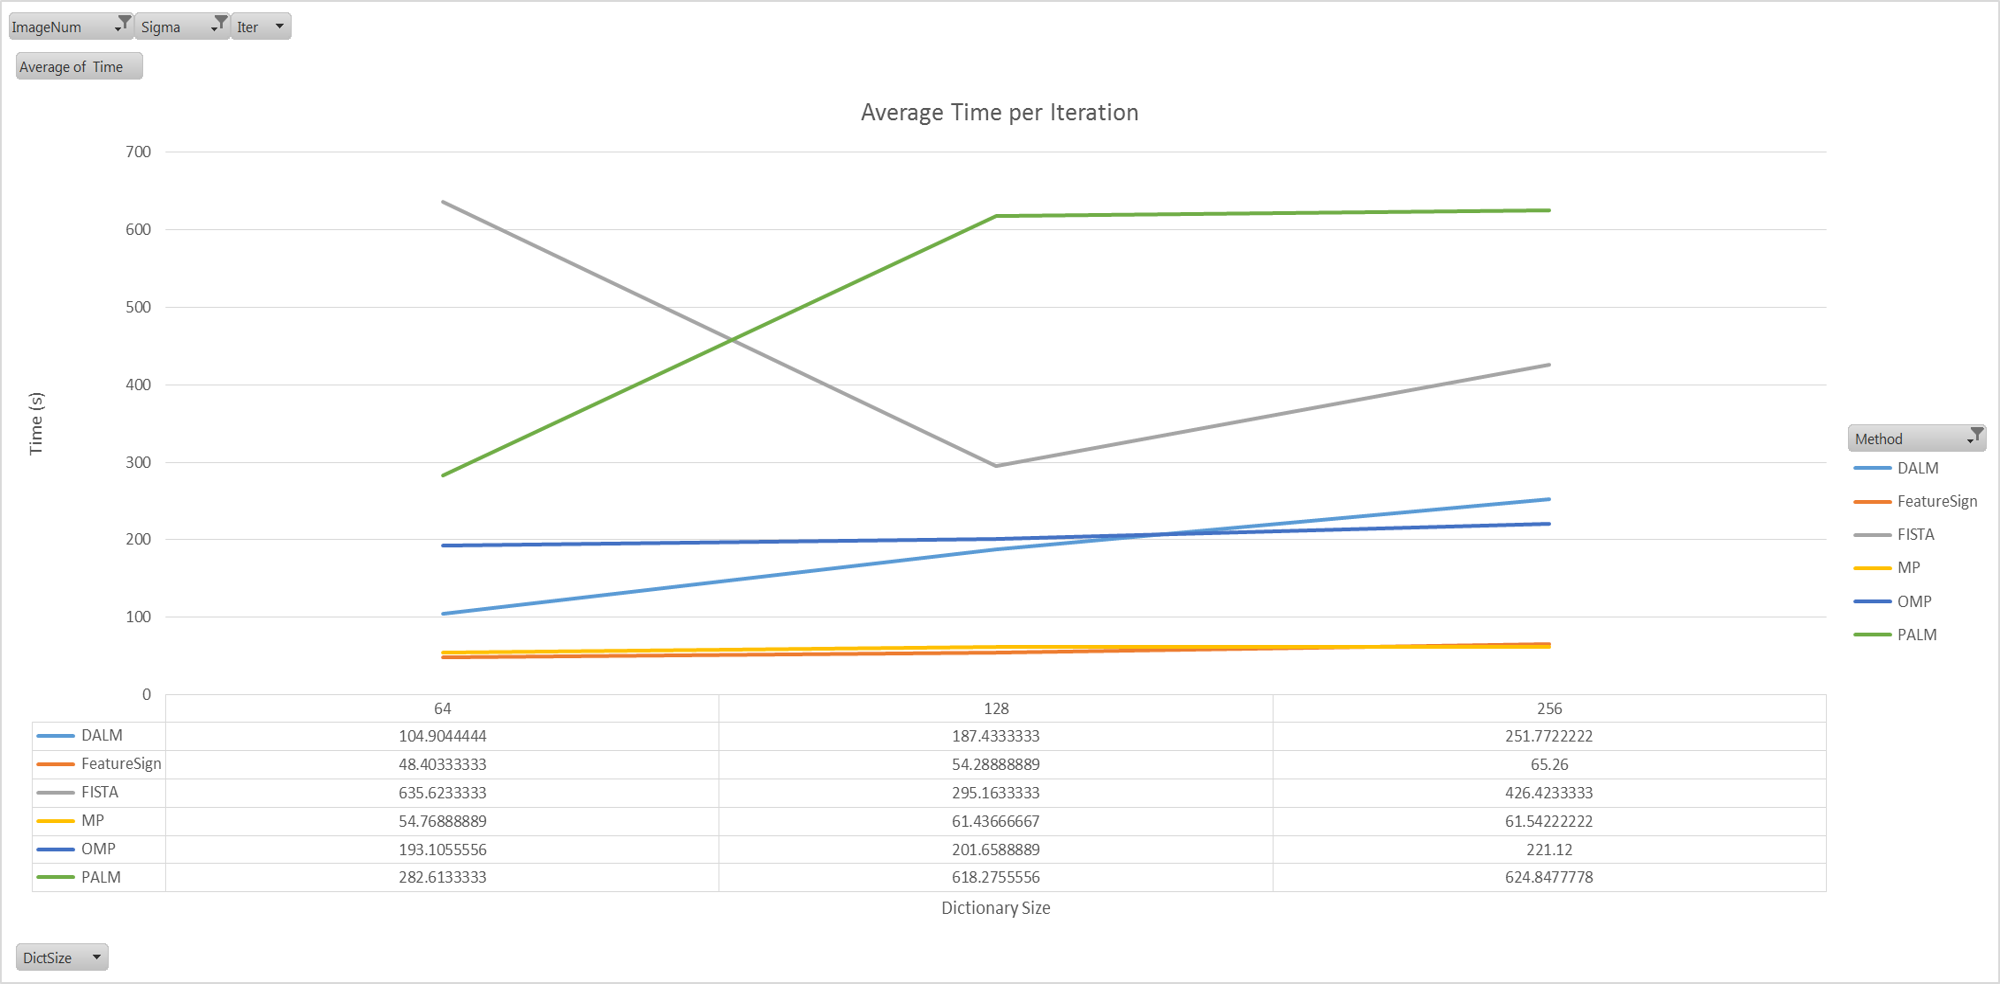
\includegraphics[width=\textwidth]{images/graph5}
    \caption{Average Time per iteration for others}
    \label{fig:avgTimeOthers}
\end{figure*}

\begin{figure*}[h]
        \centering
        \begin{subfigure}[b]{0.5\textwidth}
                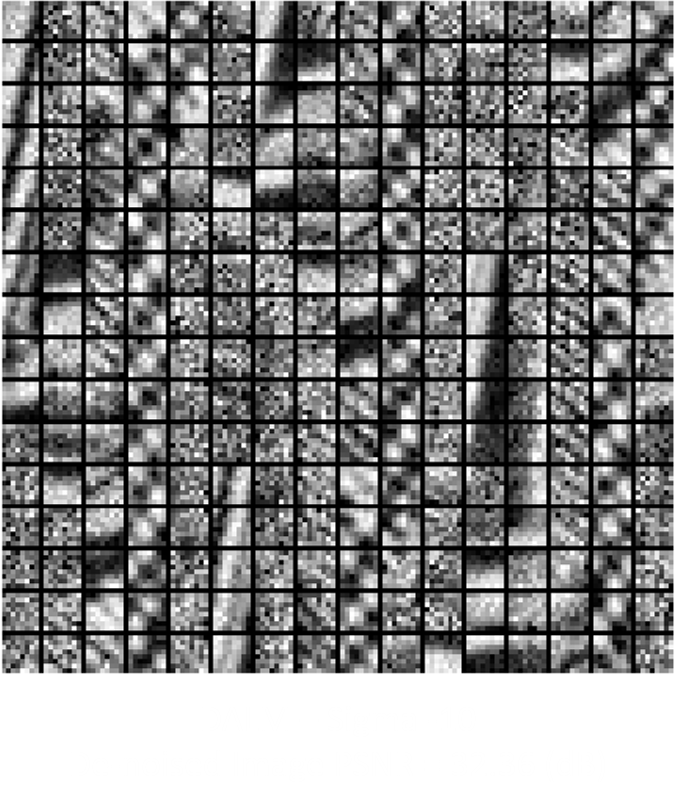
\includegraphics[width=\textwidth]{images/Trained_dict_DALM}
                \caption{Trained Dictionary for DALM\\PSNR = 32.36dB}
                \label{fig:DictDALM}
        \end{subfigure}%
        ~ %add desired spacing between images, e. g. ~, \quad, \qquad etc.
          %(or a blank line to force the subfigure onto a new line)
        \begin{subfigure}[b]{0.5\textwidth}
                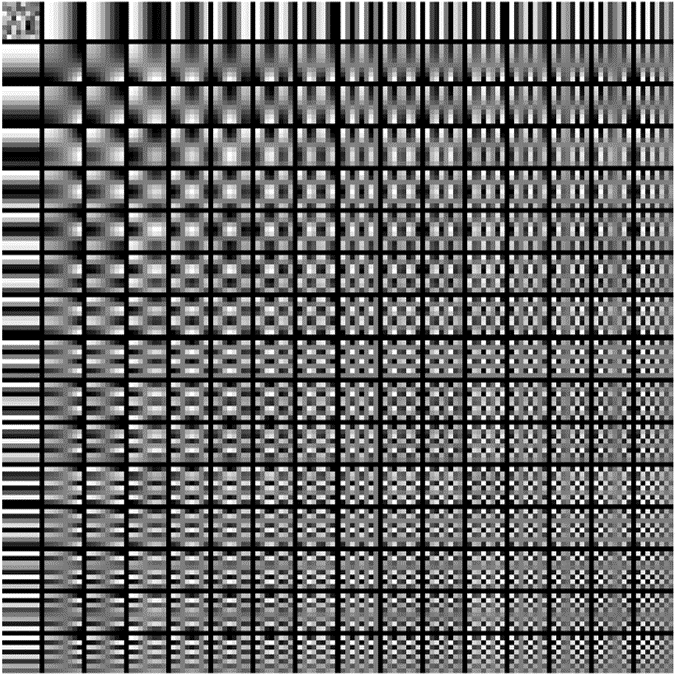
\includegraphics[width=\textwidth]{images/Trained_dict_PALM}
                \caption{Trained Dictionary for PALM\\PSNR = 33.99dB}
                \label{fig:DictPALM}
        \end{subfigure}
        \caption{Trained Dictionary}\label{fig:Dict}
\end{figure*}

\begin{figure*}[h]
        \centering
        \begin{subfigure}[b]{0.5\textwidth}
                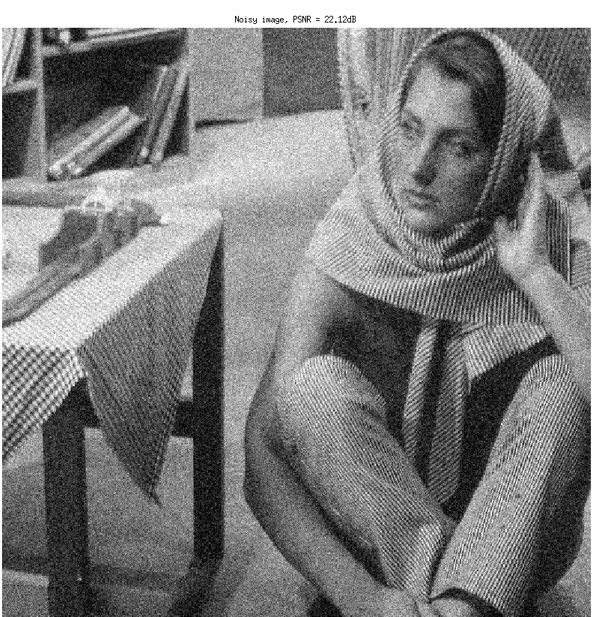
\includegraphics[width=\textwidth]{images/Noisy}
                \caption{Noisy Image\\PSNR = 22.12dB}
                \label{fig:NoisyIm}
        \end{subfigure}%
        ~ %add desired spacing between images, e. g. ~, \quad, \qquad etc.
          %(or a blank line to force the subfigure onto a new line)
        \begin{subfigure}[b]{0.5\textwidth}
                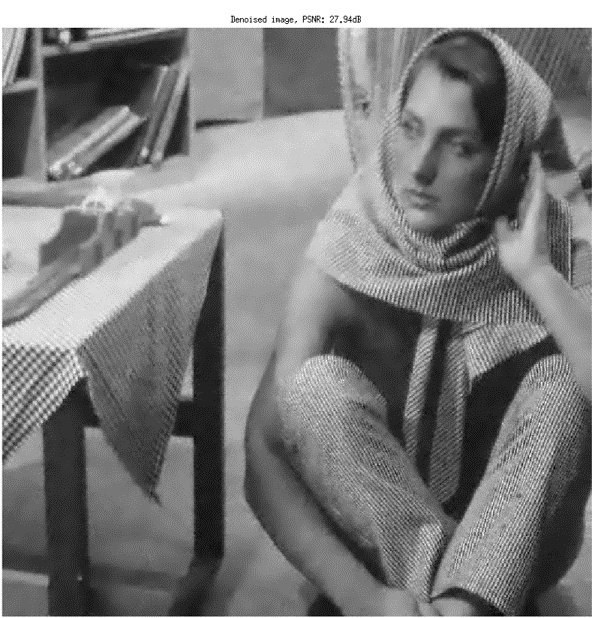
\includegraphics[width=\textwidth]{images/Denoised_DALM}
                \caption{Denoised Image for DALM\\PSNR = 27.94dB}
                \label{fig:DenoisedDALM}
        \end{subfigure}
        \caption{Images after Denoising - DALM\\Sigma = 20}\label{fig:DenoiseDALM}
\end{figure*}


\begin{figure*}[h]
        \centering
        \begin{subfigure}[b]{0.5\textwidth}
                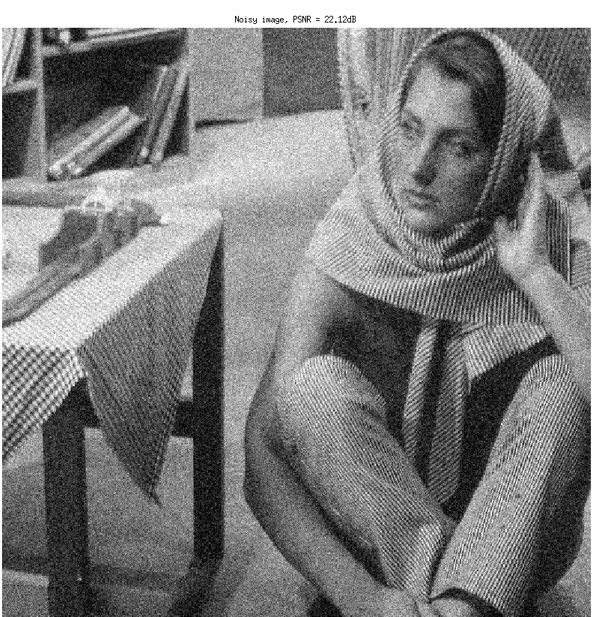
\includegraphics[width=\textwidth]{images/Noisy}
                \caption{Noisy Image\\PSNR = 22.12dB}
                \label{fig:NoisyIm}
        \end{subfigure}%
        ~ %add desired spacing between images, e. g. ~, \quad, \qquad etc.
          %(or a blank line to force the subfigure onto a new line)
        \begin{subfigure}[b]{0.5\textwidth}
                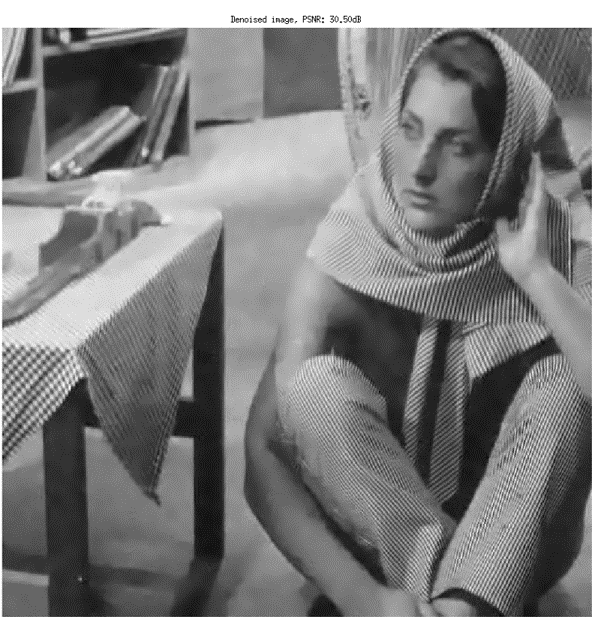
\includegraphics[width=\textwidth]{images/Denoised_FeatureSign}
                \caption{Denoised Image for FeatureSign\\PSNR = 30.50dB}
                \label{fig:DenoisedFeatureSign}
        \end{subfigure}
        \caption{Images after Denoising - Feature Sign\\Sigma = 20}\label{fig:DenoiseFeatureSign}
\end{figure*}

\vspace{.2cm}
\section{Conclusion}
\vspace{.2cm}
In this paper, we have studied the behaviour of different sparse coding techniques in K-SVD for Dictionary Learning in the Image De-noising context. We provide a comprehensive comparison of timing and de-noising performance for different sparse coding techniques over varying dictionary sizes and noise levels. We see that performance improves with increasing dictionary size. Feature-sign gives best results and converges quickerthan the other methods. L1LS takes the maximum time per iteration. DALM learns a poor dictionary.


\nocite{*}
\bibliographystyle{plain}
\bibliography{AML}

\newpage
\section{Appendix}


\subsection{Appendix-1}
\label{sec:Appendix1}
 

\subsection{Appendix2}
\label{Appendix2}



\end{document}
